\documentclass{article}
\usepackage{imakeidx}
\usepackage{graphicx}
\usepackage{wrapfig}
\usepackage{mathtools}
\graphicspath{{images/}}
\usepackage{geometry}
\geometry{a4paper,
total={170mm, 257mm},
left = 30mm,
right = 30mm,
bottom = 30mm,
top = 30mm
}

\usepackage{multicol}
\title{C/C++\linebreak Revision Notes}
\author{James Brown}
\makeindex
\begin{document}
	\pagenumbering{gobble}
	\maketitle
	\newpage
	\tableofcontents
	\newpage
	\pagenumbering{arabic}

	\section{Introduction}
	These are notes I have written in preparation of the 2017 C/C++ exam. This year the module was run by Hayo Thielecke (H.Thielecke@cs.bham.ac.uk). This module focuses on the features of C and C++ that are important in Computer Science in general. It is not a rerun of the first year Software Workshop module.
	\linebreak \linebreak
	
	\section{Pointers and Memory Management}
	\subsection{Pointers}	
	Pointers are a fundamental feature of C which have not been encountered in programming languages we have used to this point, and they are used everywhere in C. What is the meaning of \texttt{x = x + 1;}? It does not mean $2 = 2 + 1$. The \texttt{x} on the left side of the \texttt{=} refers to the address (L-value) \texttt{x}. The \texttt{x} on the right side of the \texttt{=} refers to the contents (R-value) of \texttt{x}. Here, the L-value is a \textbf{pointer}\index{pointer}
	
	\par 
	The view of memory in C is of a graph, as we would like to abstract away from actual hardware addresses. Nodes in the graph are chunks of memory (often this is a struct), and edges between nodes are pointers. Due to this, box-and-arrow diagrams are very useful in representing the state of memory.
	
	\begin{figure}[ht]
		\begin{minipage}[t]{0.45\textwidth}
			\centering
			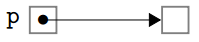
\includegraphics[width=0.45\textwidth]{box_arrow_diagram}
			\caption{A box-and-arrow diagram}
			\label{fig:bow arrow diagram}
		\end{minipage}
		\hfill
		\begin{minipage}[t]{0.45\textwidth}
			\centering
			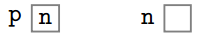
\includegraphics[width=0.45\textwidth]{box_arrow_diagram_memory}
			\caption{The hardware level of a box-and-arrow diagram}
			\label{fig:box arrow diagram memory}
		\end{minipage}
	\end{figure}	
		
	\subsubsection{The * and \& Operators}
	In C, * is also a unary operator. It is also used for binary multiplication, but the two have nothing to do with each other. If \texttt{P} is an expression denoting a pointer, then \texttt{*P} is the result of derefencing the pointer (that is getting the value of the thing it points to in memory). If \texttt{T} is a type, then \texttt{T *p;} declares \texttt{p} to be of type 'pointer to \texttt{T}'. If \texttt{T} is a type, then \texttt{T*} is the type of pointers to something of type \texttt{T} - this is used in casting. Important to note is that the \texttt{*} does not stick to everything in a declaration. For example, \texttt{int *p, n;} is like:
	
	\begin{verbatim}
	int *p;
	int n;
	\end{verbatim}
	
	and not
	
	\begin{verbatim}
	int *p;
	int *n;
	\end{verbatim}
	
	Care should be taken when defining pointers in this fashion.	
	
	\par 
	If a variable appears on the right-hand side of an \texttt{=}, its R-value is taken. If we want to get the address of a variable rather than its contents, we use the \texttt{\&} operator - \texttt{\&x} for example.
	
	\par 
	In C, two pointers are \texttt{==} if they refer to the same address in memory. Pointer equality is different from structural equality that is built into other languages. \texttt{p = q}  makes \texttt{p == q}. \texttt{*p = *q} does not make \texttt{p == q}.
	
	\subsubsection{The Null Pointer}
	There is a special pointer value, called the \textbf{null} pointer. In C, it is called the \texttt{NULL} pointer and in C++ it is called the \texttt{nullptr}. The null pointer, unsuprisingly, does not point to anything. Derefencing \texttt{NULL} will give an undefined behaviour (usually this will be a crash). In C, we have an idiom to test whether a point \texttt{p} is equal ot the null pointer:
	\begin{verbatim}
	if(p) ...
	\end{verbatim}
	
	It is important to note that pointers are not always initialised to null. 
	
	\subsection{Memory Management with \texttt{malloc} and \texttt{free}}
	In C, \texttt{stdlib.h}\index{stdlib.h} provides the functions \texttt{malloc}\index{malloc} and \texttt{free}\index{free}. The part of memory managed by \texttt{malloc} is called the \textbf{heap}\index{heap}. \texttt{malloc} allows us to borrow some memory from the memory manager, and \texttt{free} allows us to give back the memory that we have borrowed. We must promise to not use the memory that we have freed again, although the memory manager cannot force us not to do this. Regardless we still should not touch freed memory has it can lead to undefinied behaviour. Also important to note is that the call to \texttt{free} changes the ownership of the memory, not any of the pointer which pointed to that memory. The \texttt{free} operator is very important, as our program will leak memory otherwise. Luckily, we have tools such as Valgrind to help us analyse our code and test for memory errors and leaks.
	
	\par 
	\texttt{malloc} and \texttt{free} are not part of the C language itself, only its standard library. Due to this, we could implement our own memory allocator in C if we so wish. The allocator would request some memory from the OS (this would be done via \texttt{sbrk} in Unix). The available memory would be divided into chunks that are linked together in a 'free list'. A call to \texttt{malloc} will then detach a chunk from the free list and return a pointer to it. A call to \texttt{free} takes the pointer to the chunk and links it back into the free list. This is not massively efficient and may also result in memory fragmentation, but the fact we can do it is still impressive.
	
	\par 
	What happens once \texttt{free} is called upon some memory? Various things: the same piece of memory may be used again in a later \texttt{malloc}, or the memory manager might write its own data structures into the memory (e.g. the free list). Rather than trying to guess exactly what happens, we simply call it undefined behaviour. C, unlike other languages, will not prevent you from doing bad things with freed memory. 
	
	Using \texttt{malloc} and \texttt{free} we could write a piece of example code like such:
	\begin{verbatim}
	int *p1, **p2;
	p1 = malloc(sizeof(int));
	*p1 = 7;
	p2 = malloc(sizeof(int*));
	*p2 = p1;
	free(p1);
	\end{verbatim}
	
	If we add the line \texttt{**p2 = 11;} as the last line of this piece of code, we would be adding an example of use after free, which we should absolutely avoid doing!
	
	\subsubsection{The \texttt{sizeof} operator}
	For using \texttt{malloc}, we need to tell the function how many bytes to allocate. Usually, we are allocating enough memory to hold a specific type, but sizes of types are implementation dependent. The compiler will tell us how big it makes each type, and this can be found by using \texttt{sizeof(T)}. Very commonly we will write a piece of code as follows:
	
	\begin{verbatim}
	T *p = malloc(sizeof(T));
	\end{verbatim}
	
	\subsubsection{Crashes vs Memory Errors}
	In C, crashes and memory errors are not the same thing. Crashes usually have many names, such as core dumps\index{core dump} or segmentation faults\index{segmentation fault}\index{segfault}. Crashes are errors which have been detected by the hardware or the OS. In C, a memory error \textit{may} lead to a segfault, but it is not guaranteed that it will. A write error which does not lead to a segfault may instead lead to corrupted memory - this could be even worse! A C program with a memory error is always wrong. A memory leak is not the same as a memory error, and not always a bad situation. A memory leak may lead to a crash though when the program eventually runs out of memory.
	
	\section{Structures in C}
	A structure (or \texttt{struct}) is much like a Java class that contains only data and no methods. When talkinga about structures, we say that they have \textbf{members}\index{members}, not variables. In C, we cannot define functions inside a struct but we can in C++. In C, functions are defined outside of structs and often access them via pointers. Structures and pointers (along with \texttt{malloc}) lets us build many classic data structures such as lists, trees and graphs.
	
	\par 
	The syntax for C structures is very similar to the syntax of Java classes:
	
	\begin{verbatim}
	struct s {
	    T1 m1;
	    ...
	    Tk mk;
	};
	\end{verbatim}
	
	After a structure, \texttt{s}, has been declared, \texttt{struct s} can be used as a type name:
	
	\begin{verbatim}
	int n;          // declares n as an int
	struct s y;     // declares y as a struct s
	struct s *p;    // declares p as a pointer to a struct s
	\end{verbatim}	
	
	Access to structure members is done by using the dot operator, e.g. \texttt{s.m1}. Structure members are laid out in memory in order, with possibly a few bytes of padding between structure members due to alignment, depending on the hardware. For this reason, \texttt{sizeof(struct S)} $\geq$ \texttt{sizeof(T1) + ... + sizeof(Tk)}.
	
	\subsection{The $->$ operator}
	\texttt{p -> m} is an abbreviation for \texttt{(*p).m}. It defrences the pointer and then access the structure member. This operation is very, very common in C and C++ code. This operation can be chained together, for example \texttt{p->m1->m2->m3}.
	
	\par 
	This operator will be commonly used to traverse over a list like so, as C does not have an iterator idiom:
	\begin{verbatim}
	while(p) {
	    ...
	    p = p -> next;
	}
	\end{verbatim}
	
	It would be incorrect to right something like \texttt{while(p->next){...})}, as this ignores the fact that a linked list may be \texttt{null}, which represents the empty list. We should begin by testing for the \texttt{null} pointer.
	\begin{figure}
	\begin{minipage}[b]{0.48\textwidth}
	\begin{verbatim}
	while(lp) {
	    q = lp;
	    lp = lp -> next;
	    free(q);
	}
	\end{verbatim}
	\caption{A piece of code to delete all elements of a linked list}
	\end{minipage}
	\hfill
	\begin{minipage}[b]{0.48\textwidth}
	\begin{verbatim}
	while(lp) {
	    free(lp);
	    lp = lp -> next;
	}
	\end{verbatim}
	\caption{The same code with a use after free error}
	\end{minipage}
	\end{figure}
	
	\section{Pointer Arithmetic and Arrays}
	\subsection{Arrays and Strings in C}
	In C, we define an array in the same way we would define an array in Java: \texttt{char b[2];}. The size of the array is also not stored, like it is in Java, and we have to track the array bounds ourselves. When an array is passed into a function, a pointer to the start of the array must be passed - not the contents of the array. In Java, \texttt{a[i]} will either refer to the i-th element of the array or throw an index out-of-bounds exception if i is too big. In C, a[i] will either refer to the i-th element of the array or cause undefined behaviour if i is too big - this is completely undesirable behaviour. Not doing bounds checks is faster, for example: if we want to multiply two 100000 x 100000 matricies, do we really want the compiler to do a bounds check for each array access? 
	\par In C, a string is an array of char's which is terminated by a zero byte. The zero byte, \texttt{\textbackslash 0} is not the same as the character "0" (which in ASCII is 48).
	
	\subsubsection{The Arguments to Main}
	The \texttt{main} function takes two arguments: an array of strings and the number of strings there are passed like so:
	\begin{verbatim}
	main(int argc, char *argv[]) { ... }
	\end{verbatim}
	
	Should we not need the arguments, in C (but not C++) we can also write:
	
	\begin{verbatim}
	main() { ... }	
	\end{verbatim}	
	
	\subsection{Pointer Arithmetic}
	In C, we can add an integer to a pointer, but we cannot add two pointers. Array access is achieved through pointer arithmetic. When adding to a pointer, \texttt{p + 1} does not mean \texttt{p} plus one byte. Instead, in \texttt{p + n}, \texttt{n} is scaled up by the size of the type of what \texttt{p} points to. 
	
	\subsection{Buffer Overflows}
	All array access in C are potentially dangerous, and as strings in C are arrays they too are dangerous. Arrays can potentially overflow, so we should always check the bounds of the array. An example of a vulnerable function is as follows:
	
	\begin{verbatim}
	void mystrcpy(char *q, char *p) {
	    while(*q++ = *p++);
	}
	...
	char a[] = "abc";
	char b[2];
	mystrcpy(b, a);
	\end{verbatim}
	
	If we use this function with more characters than array space allocated (as shown in the above example), the function will continue to copy - even if it is overwriting other data - until it hits the zero byte in the string. Some C compilers will do some buffer overflow mitigation, but should not be relied upon. Instead, we should use functions with bounds such as \texttt{strncpy} and \texttt{fgets}. For more advanced attacks using buffer overflow attacks, we need to understand how C is compiled. If we can overwrite the return address of the function, we can alter the flow of the program. It may even be possible to `return' back to code we have injected.
	
	\subsection{First-class functions in C and C++}
	C has \textbf{pointers} to functions. In C, functions cannot be defined inside of other functions, but functions in C can be passed as a parameter very easily - they are just code pointers. If we have a function pointer \texttt{p}, then we can call it via \texttt{(*p)(...)}. We may use this in the \texttt{fold} function for example, which takes a binary operator function as an argument:
	
	\begin{verbatim}
	int fold(int n, int (*bin)(int, int), struct Linked *p) {
	    while(p) {
	        n = bin(n, p->data);
    	   p = p->next;
	    }
	    return n
	}
	\end{verbatim}
	
	\section{Typed Trees in C}
	Using what we already know, we can build n-ary trees using structures and pointers. Recursion in these trees ends by \texttt{null} pointers, hence the \texttt{if(p)} and \texttt{while(p)} idioms. These trees only have one kind of node, which may be sufficient for some situations. In Computer Science, we have more complex trees with different kinds of nodes with different numbers and kinds of child nodes. These trees need a different type system of different numbers. The most common example of these kinds of trees is \textbf{abstract syntax trees}\index{abstract syntax trees}. These are fundamental for compilers.
	
	\subsection{\texttt{struct}, \texttt{union} and \texttt{enum}}
	Using what we have, we cannot represent typed trees such as abstract syntax trees very easily. The addition of \texttt{union} and \texttt{enum} can make doing this much easier. 
	
	\subsubsection{\texttt{union}}
	The syntax of \texttt{union} is like that of \texttt{struct}. 
	
	\begin{verbatim}
	union u {
	    T1 m1;
	    T2 m2;
	    ...
	    Tk mk;
	};
	\end{verbatim}
	
	We can think of unions as a choice between any of the members. The official C11 draft standard says in section 6.7.2.1 that a union is a type consisting of a sequence of members whose storage overlap. Unions are not tagged, so the memory does not know whether is contains data of type \texttt{T1} or type \texttt{T2}. If we want a tagged union, we need to enclose the \texttt{union} within a \texttt{struct} with a \texttt{enum}
	
	\subsubsection{\texttt{enum}}
	\texttt{enum} is the enumeration type, much like as it is in Java. 
	
	\begin{verbatim}
	enum dwarf { thorin, oin, gloin, fili, kili };
	\end{verbatim}

	In it's implementation small integers are used, for example \texttt{thorin = 0} and so on.
	
	\subsubsection{Tagged unions idiom}
	We will use an \texttt{enum} as the tag for our union. We then package the \texttt{union} in a \texttt{struct} along with the \texttt{enum}.
	
	\begin{verbatim}
	enum ABtag { isA, isB };
	
	struct taggedAorB {
	    enum ABtag tag;
	    union {
	        A a;
	        B b;
	    } AorB;
	};
	\end{verbatim}
	
	Here the \texttt{struct} can either be A or B, and we know which it will be by looking at the tag in the \texttt{enum}. We can access the tagged unions with \texttt{switch}:
	
	\begin{verbatim}
	struct taggedAorB x;
	...
	switch(x.tag) {
	    case isA:
	        // use x.AorB.a
	    case isB:
	        // use x.AorB.b
	}
	\end{verbatim}
	
	\par Having to invent names for \texttt{struct}, \texttt{union} and \texttt{enum} members can be tedious. We may wish to use a systematic naming scheme for a given situation and stick to it, but this is a matter of taste. Since C11, we can use anonymous \texttt{struct}s and \texttt{union}s, like so:
	
	\begin{verbatim}
	struct s2 {
	    struct t2 { int q; ... } ;
	    int n;
	}
	\end{verbatim}

	The inner \texttt{struct} is anonymous by lacking a member name, but the compiler still knows what \texttt{q} is.

	
	\subsection{Typed Trees}
	We have explored how to create tagged \texttt{union}s, which can be processed with a \texttt{switch} statement. If we add pointers and recursion, we can create \textbf{typed trees}\index{typed tree}. From trees a pointers, we can also get \textbf{graphs}\index{graph}
	
	\subsubsection{Trees with values only at the leaves}
	\begin{verbatim}
	enum treetag { isLeaf, isInternal } tag;
	
	struct intbt {
	    enum treetag tag;
	    union {
	        // if tag == isLeaf, use this:
	        int Leaf; // no recursion
	        // if tag == isInternal, use this:
	        struct {
	            struct intbt *left;     // recursion
	            struct intbt *right;    // recursion
	        } Internal;
	    } LeafOrInternal;
	};
	\end{verbatim}	
		
	This is not the same as a tree using \texttt{struct} and pointers. A tree built like such would require \texttt{null} pointers to terminate. As our abstract syntax trees are not supposed to contain null pointers at all, we would like to ensure that this is the case. We can use the \texttt{assert} macro from \texttt{assert.h}. \texttt{assert(p)} means that we are not expecting a null pointer in \texttt{p}. An error will be thrown if the assertion fails. We can use assertions in debugging, and turn them off in production code. 
	
	\subsubsection{AST for Lisp-style expresions}
	
	\begin{figure}[ht]
		\begin{minipage}[t]{0.45\textwidth}
		\caption{A grammar for a Lisp-style language}
		\begin{align*}
		&E \rightarrow n  &\text{(constant)} \\
		&E \rightarrow x  &\text{(variable)} \\
		&E \rightarrow (+ L)  &\text{(addition)} \\
		&E \rightarrow (* L)  &\text{(multiplication)} \\
		&E \rightarrow (= x E E)  &\text{(let binding)} \\
		&L \rightarrow E L	 &\text{(expression list)} \\
		&L \rightarrow		&\text{(empty list)}
		\end{align*}
		\end{minipage}
		\hfill
		\begin{minipage}[t]{0.45\textwidth}
		\caption{The abstract syntax tree of this language}
		\begin{verbatim}
		enum op {isplus, ismult};
		enum exptag {islet, isconstant, isvar, isopapp};
		
		struct exp {
		    enum exptag tag;
		    union {
		        int constant;
		        char var[8];
		        struct {
		            enum op op;
		            struct explist *exps;
		        }; // anonymous struct
		        struct {
		            char bvar[8];
		            struct exp *bexp;
		            struct exp *body;
		        }; // anonymous
		    }; // anonymous
		};
		
		struct explist {
		    struct exp *head;
		    struct explist *tail;
		};
		\end{verbatim}
		\end{minipage}			
	\end{figure}		
		
	
	\section{From C and Java to C++}
	By now, we have covered all of the most important contructs of the C programming language. We now move to C++. C++ aims to be as efficient as C, but with more structure to the language. It is both a high-level and a low-level language, without garbage collection. C++ also has object orientation, but you are not forced to use it.
	
	\subsection{Virtual Functions}
	\begin{itemize}
		\item \textbf{Non-Virtual}: the compiler determines from the type what function to call at compile time
		\item \textbf{Virtual}: what function to call is determined at run-time from the object and its run time class
	\end{itemize}
	
	At runtime, each object of a class with virtual functions contains an additional pointer to the virtual function table (vtable). Take these two examples:
	
	\begin{verbatim}
		class Animal {
		public: void speak() { std::cout << "Noise\n"; }
		// not virtual
		};
		
		class Pig : public Animal {
		public: void speak() { std::cout << "Oink!\n"; }
		};
		
		int main(int argc, char *argv[]) {
		    Animal *peppa = new Pig();
		    peppa->speak();
		    // the type of peppa is Animal
		}
	\end{verbatim}		
	
	\begin{verbatim}
		class Animal {
		public: virtual void speak() { std::cout << "Noise\n"; }
		};
		class Pig : public Animal {
		public: void speak() { std::cout << "Oink!\n"; }
		};
		int main(int argc, char *argv[]) {
		    Animal *peppa = new Pig();
		    peppa->speak();
		    // peppa points to an object of class Pig
		}
	\end{verbatim}
	
	In the both examples, we have defined the type of peppa to be an animal, and then instantiated it as a pig. The first example uses a non-virtual function. At compile time, the compiler checks the type of peppa and sees it is an animal. Therefore, when \texttt{speak()} is called, "Noise" is printed. In the second example, \texttt{speak()} is a virtual method in \texttt{Animal}.  When \texttt{speak()} is called at run-time, what function to call is determined by the object and its run-time class, which is  \texttt{Pig}. For this reason, "Oink" is printed.
	
	\par This is a very simple example, and we could in theory make the compiler deduce the type of peppa as it is only ever instaniated to a pig, and never changed. In this example, the code will be less efficient for no real gain as it has to pass around the vtable and check the correct function to call in the virtual example. However, take the following example:
	
	\begin{verbatim}
	Animal *ap;
	if(...) {
	    ap = new Baboon();
	else
	    ap = new Weasel();
	ap->speak();
	\end{verbatim}
	
	Now it would not be so easy to predetermine the type of ap at compile-time, which shows the value of virtual functions. Whether ap points to being a baboon or a weasel will only be known at run-time.
	
	\subsubsection{Pure Virtual Functions}
	A pure virtual function has no implementation in the base class. This has a slightly peculiar notation: 
	
	\begin{verbatim}
	class C {
	    public:
	    virtual T1 f(T2) = 0; // declare f as pure virtual
	    ...
	}
	\end{verbatim}
	
	This does not suggest anything is equal to zero, the \texttt{= 0} is supposed to suggest that something is missing. Any derived classes of C should implement \texttt{f}. For example, we could have said that there is really a noise that any animal can make and we could have defined it as a pure virtual function: \texttt{public: virtual void speak() = 0;}
	
	\par 
	Furthermore, we could use pure virutal functions in our abstract syntax tree example. Each of the nodes in the tree would be an object (instance of a class) with their pointers to any children nodes. Each node would use the evaluation function of its own class, removing the need for a switch statement. This is dynamic `polymorphism' via virtual functions.
	
	\subsection{New and Delete}
	C has \texttt{malloc} and \texttt{free} for heap allocation and deallocation. C++ has \texttt{new} and \texttt{delete} fo heap allocation and deallocation. We can also define \textbf{constructors} (not surprising) and \textbf{destructors} (somewhat surprising) in C++.
	
	\par 
	C++ destructors for some class \texttt{A} are called \texttt{~A}. We do not call destructors directly, we let our call to \texttt{delete} do it implicitly. The clean-up done by the destructor may involve deleting other objects `owned' by the object to be deleted. For example, if we delete the root of a tree, we would possbily want to recursively delete all of the child nodes as well. We may also perform other resource management in a destructor such as closing any opened files.
	
	\subsection{Strings in C++}
	C uses 0-terminated character arrays as strings, which is full of pitfalls like buffer overflows and off-by-one bugs. C++ has a dedicated string class which can be used.
	 
	\section{Templates in C++}
	Templates are very similar to generics in Java. There are two kinds of templates in C++: \textbf{class templates}\index{class template} and \textbf{function templates}\index{function template}. Roughly, these correspond to polymorphic data types and polymorphic functions in functional languages. The syntax is as follows:
	
	\begin{verbatim}
	template<class T>
	class Linked {
	public:
	    T head;
	    Linked<T>* tail;
	};
	\end{verbatim}
	
	\subsection{Type inference and auto}
		
	\newpage
	\listoffigures
	\printindex
\end{document}
